\documentclass[a4paper,norsk, 10pt]{article}
\usepackage[utf8]{inputenc}
\usepackage{verbatim}
\usepackage{listings}
\usepackage{graphicx}
\usepackage[norsk]{babel}
\usepackage{a4wide}
\usepackage{color}
\usepackage{amsmath}
\usepackage{float}
\usepackage{amssymb}
\usepackage[dvips]{epsfig}
\usepackage[toc,page]{appendix}
\usepackage[T1]{fontenc}
\usepackage{cite} % [2,3,4] --> [2--4]
\usepackage{shadow}
\usepackage{hyperref}
\usepackage{titling}
\usepackage{marvosym }
\usepackage{subcaption}
\usepackage[noabbrev]{cleveref}
\usepackage{cite}
\usepackage{tikz}
\usepackage[a4paper]{geometry}

\usepackage{pgf,tikz}
\usepackage{mathrsfs}
\usetikzlibrary{arrows}


\setlength{\droptitle}{-10em}   % This is your set screw

\setcounter{tocdepth}{2}

\lstset{language=c++}
\lstset{alsolanguage=[90]Fortran}
\lstset{alsolanguage=Python}
\lstset{basicstyle=\small}
\lstset{backgroundcolor=\color{white}}
\lstset{frame=single}
\lstset{stringstyle=\ttfamily}
\lstset{keywordstyle=\color{red}\bfseries}
\lstset{commentstyle=\itshape\color{blue}}
\lstset{showspaces=false}
\lstset{showstringspaces=false}
\lstset{showtabs=false}
\lstset{breaklines}
\title{FYS2130 Oblig 10}
\author{Daniel Heinesen, daniehei}
\begin{document}
\newgeometry{left = 0cm, bottom = 0cm, top = 0cm, right = 0cm}
\begin{tikzpicture}[]
\node at (0,0) {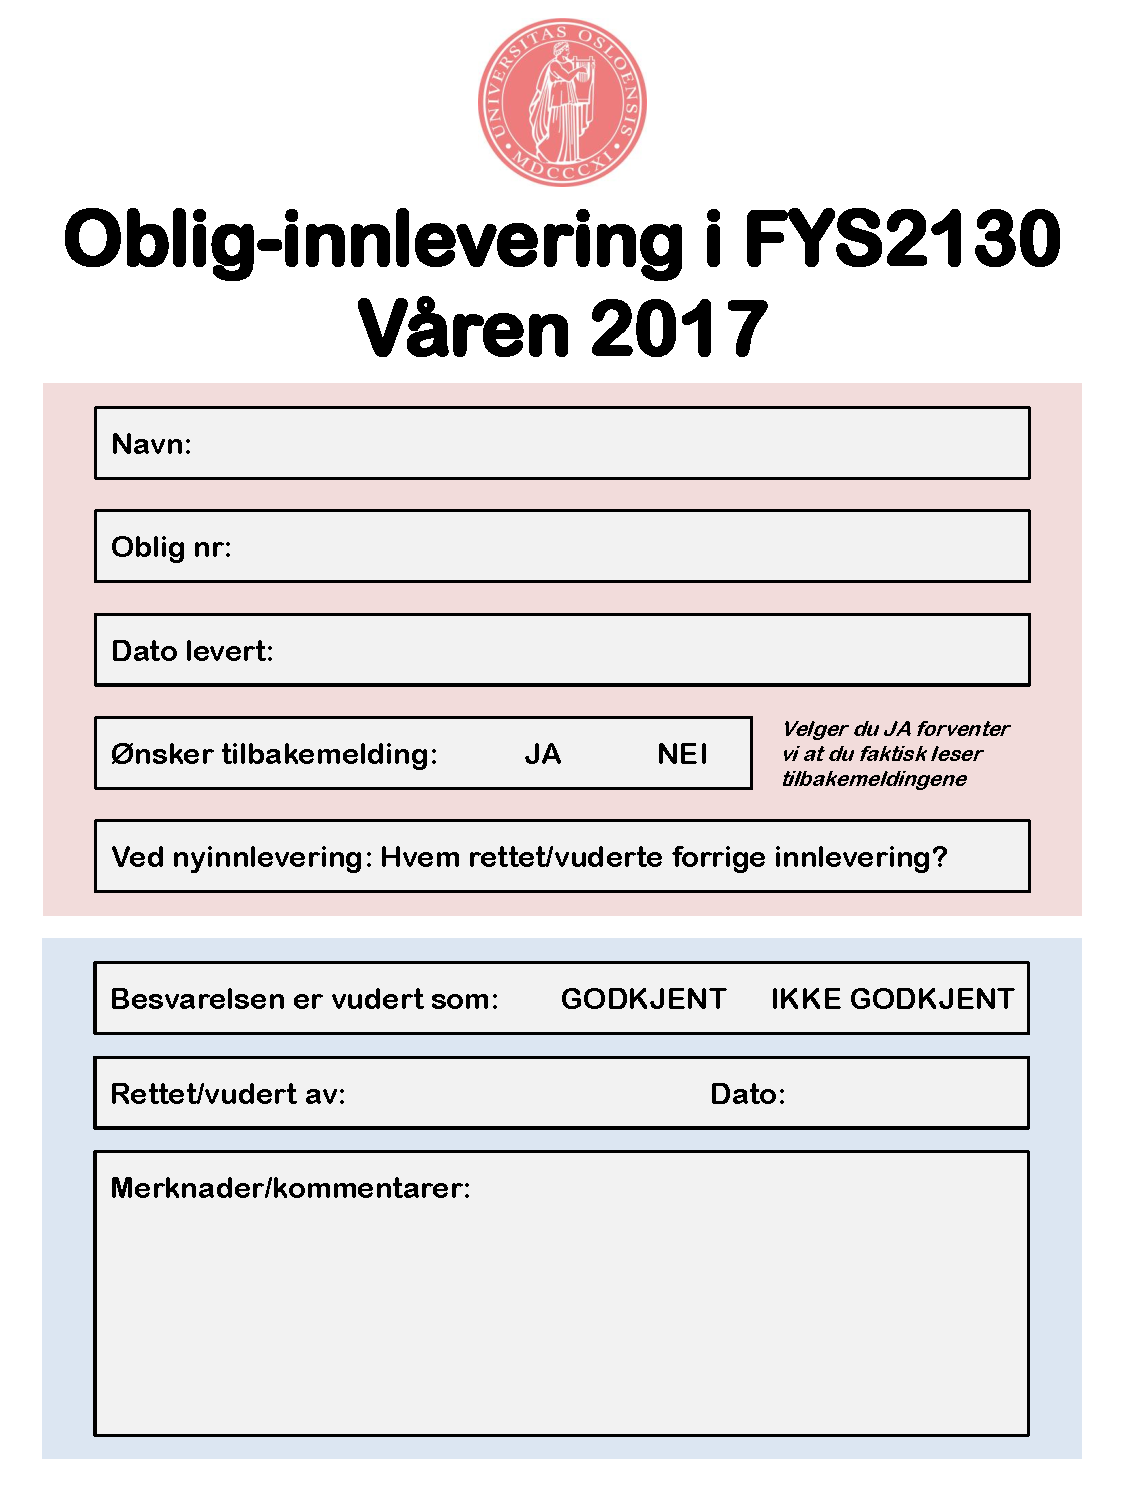
\includegraphics[width=\textwidth]{oblig_forside_2017.pdf}};
\node[right] at (-7,5.7) {\begin{huge} Daniel Heinesen \end{huge}};
\node[right] at (-6.3,3.77) {\begin{huge} 9 \end{huge}};
\node[right] at (-5.4,1.85) {\begin{huge} 04.04.2017 \end{huge}};
\draw(2.25,-0.05) circle[radius = 0.6cm];
\end{tikzpicture}


\maketitle


\section*{Oppgave 8)}

Vi vet at for en konveks linse vil et objekt bli forstørret om $s < 2f$ og forminsket om $s>2f$. Vi kan derfor bestemme brennvidden ved å se når denne overgangen mellom forstørrelse og forminskelse skjer. Vi vet da at dette er 2 ganger brennvidden.\\

En konkav linse vil alltid danne et virtuelt bilde som er mindre enn objektet. Vi kan derfor ikke bruke metoden over til å bestemme brennvidden.

\section*{Opppgave 11)}

Når lys går fra luft og inn i øyet vårt vil det bøyes litt pga forskjellige brytningsindekser. Dette er øynene våre vant til og korrigerer for dette. Hornhinnen vår har nesten samme brytningsindeksen som vann, så når vi ser under vann skjer ikke den samme bryningen som øynene våre er vant med, og vi ser derfor uskarpt. Glasset og luftlaget i dykkebillene forhindrer dette. Dette er fordi lyset ikke blir like mye brutt når det går inn i glasset. Når det går ut av glasset og mot øynene blir det derimot brutt noe. Dette gjør at ting virker større undervann. Selv om ting ser noe større ut kan vi likevel se klart undervann med dykkerbriller.\\

Uten dykkerbriller vil brytningen mellom vannet og øynene gjør at uskarpheten vi ser tilsvarer å være langsynt. Vi kan derfor bruke en konveks linse/brille når vi er under vann og få nesten samme effekt som dykkerbrillne.

\section*{Oppgave 15)}

\begin{figure}[H]
\centering
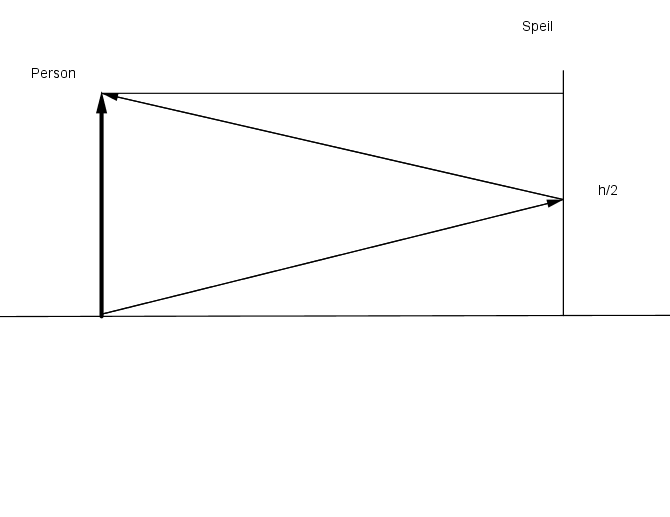
\includegraphics[scale=0.7]{speil.png}
\caption{Et speil og en person med høyde $h$. Lyset fra beina treffer speilet halvveis oppe og reflekteres tilbake og til øynene til personen. Lyset fra ansiktet går rett frem, reflekteres tilbake og går tilbake igjen til øynene.}
\end{figure}



Fra figuren over viser hvordan lyset går fra personen til speilet og tilbake. Jeg har bare tatt med de 2 ektremalpunktene: beina og hode. Lyset fra hode går rett frem, reflekteres av speilet og går tilbake samme vei. Dette lyset vil alltids gjør dette uavhenging av lengden fra speilet. Lyset fra beina reflekteres av speilet i høyden $h/2$, og går så til øynene til personen.\\

Dette er uavhenging av lengden fra speilet. Så lyset fra beina treffer alltid speilet i $\underline{\underline{h/2}}$. Derfor må et speil være halvparten av høyden til personen om han skal se seg selv i speilet.


\section*{Oppgave 17)}

\begin{figure}[H]
    \centering

    \begin{subfigure}[b]{0.47\textwidth}
        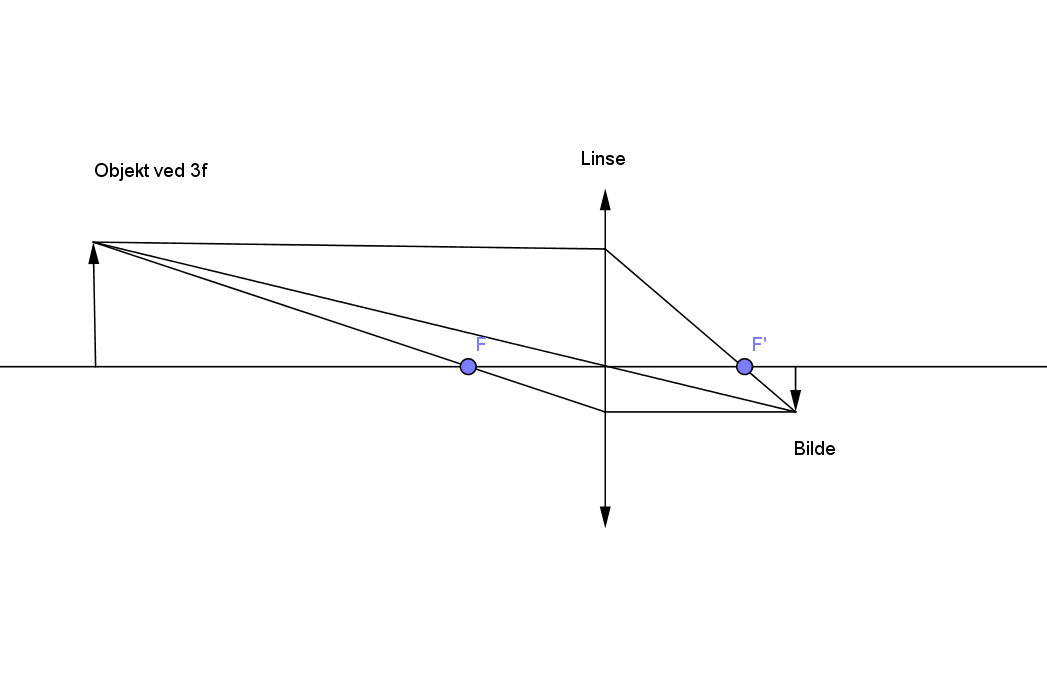
\includegraphics[width=\textwidth]{3f.png}
        \caption{Objektet er 3f unna linsen. Vi ser at vi får en forminsket bilde.}
        \label{fig:3f}
    \end{subfigure}
    ~ 
    \begin{subfigure}[b]{0.47\textwidth}
        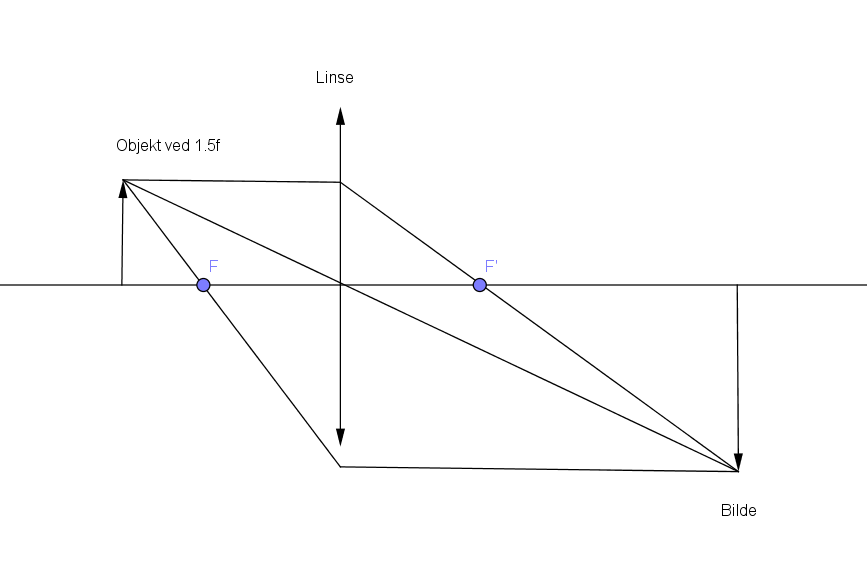
\includegraphics[width=\textwidth]{15f.png}
        \caption{Objektet er 1.5f unna linsen. Siden vi nå er mellom 1 og 2f unna linser kan se at vi får en forstørrelse av bildet.}
        \label{fig:15f}
    \end{subfigure}
    ~ 
    \begin{subfigure}[b]{0.47\textwidth}
        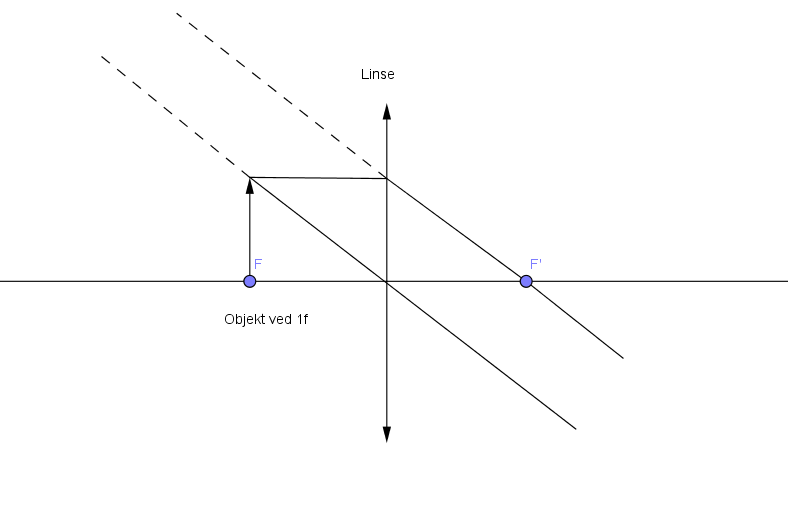
\includegraphics[width=\textwidth]{1f.png}
        \caption{Objektet ligger nå akkurat i brennvidden til linsen. Dette gjør at alle lysstrålene er parallelle på høyresiden av linsen. Vi trenger derfor bare to lysstråler -- objektet er i brennpunktet, noe som gjør at vi ikke kan tegne en ståle fra objektet og ned i $f$--. Vi får nå et virtuelt bilde som er uendelig lang foran linsen.}
        \label{fig:1f}
    \end{subfigure}
     ~ 
    \begin{subfigure}[b]{0.47\textwidth}
        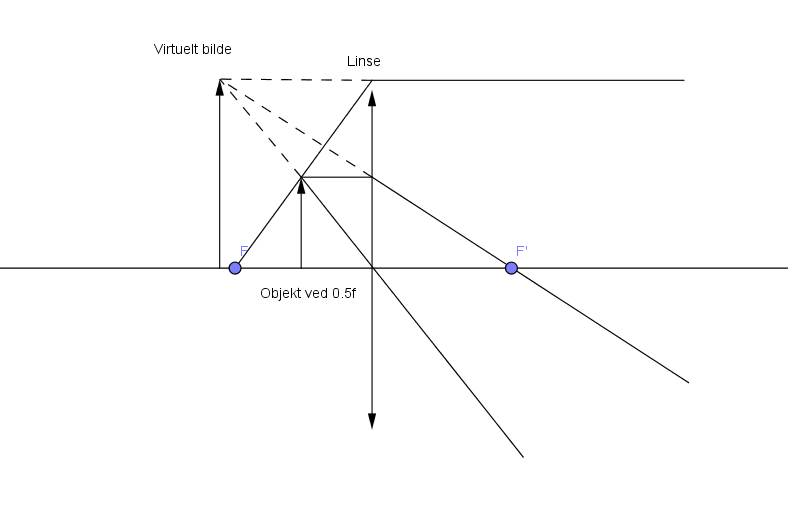
\includegraphics[width=\textwidth]{05f.png}
        \caption{Objektet er 0.5f unna linsen. Vi får her et forstørret virtuelt bilde foran linsen. Dette er derfor en lupe.}
        \label{fig:05f}
    \end{subfigure}
    \caption{Fire forskjellige lysstrålediagram.}\label{fig:diagram}
\end{figure}

\newpage

\section*{Oppgave 23)}

Vi har et kamera med en 85 mm linse. Vi skal ta bilde av en person som er 3.5 m unna, og lurer på avstanden mellom linsen og bildeplaten. Vi vet at definisjonen av brennvidde er 

\begin{equation}
\frac{1}{f} = \frac{1}{s} + \frac{1}{s'}
\end{equation}

Vi er interesserte i $s'$:

$$
 \frac{1}{s'} = \frac{1}{f} - \frac{1}{s} = \frac{1}{0.085} - \frac{1}{3.5}
$$

Dette gir oss at bildeplaten er $\underline{\underline{87.1}}$ mm bak linsen.\\

Vi har en 24 x 36 mm CMOS bildeplate, og lurer på om hele personen på 1.75 m kommer med på bildet. Forstørrelsen til bildet er gitt ved

\begin{equation}
M = -\frac{s'}{s} = -\frac{0.0085}{3.5} = -0.0243
\end{equation}

Forstørrelsen er negativ, som betyr at bildet er oppned. Vi kan fra dette finne høyden på bildet:

\begin{equation}
h = M \cdot 1.75m = 42.5 \text{ mm}
\end{equation}

Siden bildeplaten bare er 36 mm høy for vi \textbf{ikke} plass til hele personen på bildet.\\

Har vi en bildeplate som er 15.8 x 23.6 mm for vil bare plass til 

$$
\frac{23.6 \text{ mm}}{42.5 \text{ mm}} = 0.56
$$

Vi får derfor bare plass til $\underline{\underline{56 \%}}$ av personen på bildet.

\section*{Oppgave 25)}

Vi skal se på mars med en konkave linse. Konkave linser han bare virtuelle bilder. Vi har en 1000 mm linse. Mars er 6796 km bred og ligger $5.58 \cdot 10^7$ km unna jorden. Vi kan finne forstørrelsen som 

\begin{equation}
M = -\frac{s'}{s} 
\end{equation}


Hvor 

$$
s' = \frac{1}{\frac{1}{f}-\frac{1}{s}} = \frac{1}{\frac{1}{1000 \text{ mm}}-\frac{1}{5.58 \cdot 10^7 \text{ km}}} = 1000.00000002 \text{ mm}
$$

Siden vi har en konkave linse får vi et viruelt bilde, og derfor blir $s' = -1000.00000002$ mm. Vi kan så finne forstørrelsen

$$
M = 1.79211469537e-11
$$

Dette gir oss at det virtuelle bildet år en størrelse på 

\begin{equation}
h_v = M\cdot 6796 \text{ km}= 0.000122 m
\end{equation}

Bildet er altså $\underline{\underline{0.122}}$ mm stort. Her kan det være en del numerisk feil i beregningene. For en konkav linse vil innkommende parallelle lysstråler gi et viruelt bilde med høyde $\approx 0$. Mars er såpass langt unna at lysstrålene mer eller mindre er parallelle, men ikke helt. Derfor får vi en ikke-null høyde, men som er veldig liten.

\section*{Oppgave 30)}
\subsection*{a)}

Vanligvis skal nærpunket ligge på 25 cm, noe som gir n dioptre på 54. personen har nå en total linsstryke på 54 - 2.75 dioptre. Vi finner nærpunktet ved 

\begin{equation}
\frac{1}{f} = \frac{1}{x} + \frac{1}{0.02 \text{ m}} = 54 - 2.75 \text{ dioptre}
\end{equation}



Vi finner da at nærpunktet $x = \underline{\underline{80}}$ cm.

\subsection*{b)}

Vanligvis ligger fernpunktet ved uendelig, noe som gir 50 dioptre. Personene har nå en total linsestryke på 50 -(-1.3) dioptre. Vi finner da fjernpunktet 

\begin{equation}
\frac{1}{x} + \frac{1}{0.02 \text{ m}} = 51.3 \text{ dioptre}
\end{equation}
Vi finner da at fjernpunktet $x = \underline{\underline{77}}$ cm.


\section*{Oppgave 32)}
En person har et nærpunkt på 75 cm og et fjernpunkt på 3 m.\\

Vi starter med nærpunket. Vanligvis skal nærpunktet ligge på 25 cm. Dette gir en linsestyrke på 54 dioptre. Ved et nærpunkt på 30 cm vil linsestyrke på

\begin{equation}
\frac{1}{f} = \frac{1}{0.75} + \frac{1}{0.02} = 51.3 \text{ dioptre}
\end{equation}

For å rette på nærpunktet trenger personen en akkomodasjon på \underline{\underline{2.7}} for nå den normale 54 dioptre.\\

Fjernpunktet ligger vanligvis ved uendelig. Dette gir en linsestyrke på 50 dioptre. Personen har et fjernpunkt på 3 m, dette gir en linsestyrke på

\begin{equation}
\frac{1}{f} = \frac{1}{3} + \frac{1}{0.02} = 50.3 \text{ dioptre} 
\end{equation}

For å rette på nærpunktet trenger personen en akkomodasjon på \underline{\underline{-0.3}} for nå den normale 50 dioptre.\\

Personen må derfor ha briller med en akkomodasjon på både -0.7 og 2.3 dioptre.

\section*{Oppgave 40)}

Vi har et mikroskop med et objektiv med brennvidde på 8.0 mm, et okular med brennvidde på 18 mm. Disse er 19.7 cm fra hverandre.

\subsection*{a)}

Objektet vi skal se på legges vilkårlig nært brennpunktet til objektivet. Vi sier derfor at denne er avstanden er brennvidden til objektivet

\begin{equation}
s_1 = \underline{\underline{8 \text{ mm}}}
\end{equation}

\subsection*{b)}

Bildet fra objektivet dannes i brennpunktet til okularet. Dette betyr at $s_1'$ må være lengden mellom objektivet minus brennvidden til okularet.

\begin{equation}
s_1' = 0.197 - 0.018 = 0.179 \text{ m}
\end{equation}

Vi kan nå finne forstørrelsen til objektivet:

\begin{equation}
M_1 = \frac{s_1'}{s_1} =\frac{0.179}{0.008} = 22.375
\end{equation}

Så objektivet alene forstørrer objektet \underline{\underline{22.4 x}}

\subsection*{c)}

Okularet gjør at lysstrålene går parallelt. Disse går så inn i øyet. Siden øyet er $25$ cm langt får vi en forstørrelse på

\begin{equation}
M_2 = \frac{25 \text{ cm}}{f_2} =  \frac{25 \text{ cm}}{18 \text{ mm}} = 13.89
\end{equation}

Så okularet alene forstørrer objektet \underline{\underline{13.9 x}}

\subsection*{d)}
For et mikroskop er den totale forstørrelsen gitt ved

\begin{equation}
M_{total} = \frac{25 \text{ cm } \cdot s_1'}{f_2 s_1}
\label{eq:mikro}
\end{equation}

\subsection*{e)}

Vi bruker nå \eqref{eq:mikro} til å finne den totale forstørrelsen til mikroskopet:

\begin{equation}
M_{total} = \frac{25 \text{ cm } \cdot 17.9  \text{ cm }}{18  \text{ mm } \cdot 8  \text{ mm}} = 310.8
\end{equation}


Så mikroskopet forstørrer objektet \underline{\underline{311 x}}

\end{document}

